\section{New formalism}

The new formalism must allow simple interactions between user readable data and ifficient construction of the RBA problem. The data is going to be written is XML format, inspired by SBML standards.

\subsection{Final differences between RBAv01 and new formalism}

\begin{table}[!h]
  \centering
  \begin{tabular}{|l|c|c|c|c|}
    \hline
           & RBAv01 & RBAv01 & RBAnew \\
           & mat12  & mat15  & python \\
    \hline
    Input files & \multicolumn{2}{c|}{Custom files} & XML files \\
    & \multicolumn{2}{c|}{+ partially hard coded} & (nothing hard coded) \\
    \hline
    Code length & \multicolumn{2}{c|}{$\simeq 3500$} & $\simeq 2000$ \\
    (commented) & \multicolumn{2}{c|}{($\simeq 1000$)} & ($\simeq 500$) \\
    \hline
    Parsing & 15s & 8s & $<1$s \\
    \hline
    Solving (23 rounds) & 15s & 5s & $<2$s \\
    \hline
    1 matrix update & 580ms & 100ms & 3-10ms \\
    \hline
    1 CPLEX round & 50ms & 58ms & 30ms \\
    \hline
  \end{tabular}
  \caption{Comparison between original algorithm (RBAv01) and new formalism (RBAnew). Because performance for the old algorithm depended on matlab version, we included performance for matlab R2012a (mat12) and R2015b (mat15).}
  \label{tab:new_old_comparison}
\end{table}

\reftabt{tab:new_old_comparison} shows the main differences between RBAv01 and the new algorithm. The new algorithm uses generic XML files and is thus easier to modify for the end user. Using python, we could improve both parsing and solving time, which are significantly lower than the original algorithm.

\subsection{Input data}
Data files are described in Appendix~\ref{sec:rba_xml}.

\subsection{From data to matrices}

\paragraph{Algorithm overview}
\reffigt{fig:algo_rba_new} shows the blocks that are used to build the final matrices.
\begin{figure}[ht]
  \centering
  \includegraphics[width=\linewidth]{algo_RBA_new}
  \caption{Blocks that need to be assembled in the new algorithm.}
  \label{fig:algo_rba_new}
\end{figure}

\paragraph{Stoichiometry matrix} The procedure is standard, we will not illustrate it here. However, note that external metabolites are removed from the metabolite pool.

\paragraph{Density limits} These values are simply extracted from RBAParameters and assembled into a vector (one coefficient per compartment).

\paragraph{Species matrices} \reffigt{fig:species_matrices} shows how macromolecules are breaken down into matrices describing their composition, processing cost and weight. In the end, they are merged into a single matrix describing composition, processing cost and weight of all metabolites and macromolecules.
\begin{figure}[ht]
  \centering
  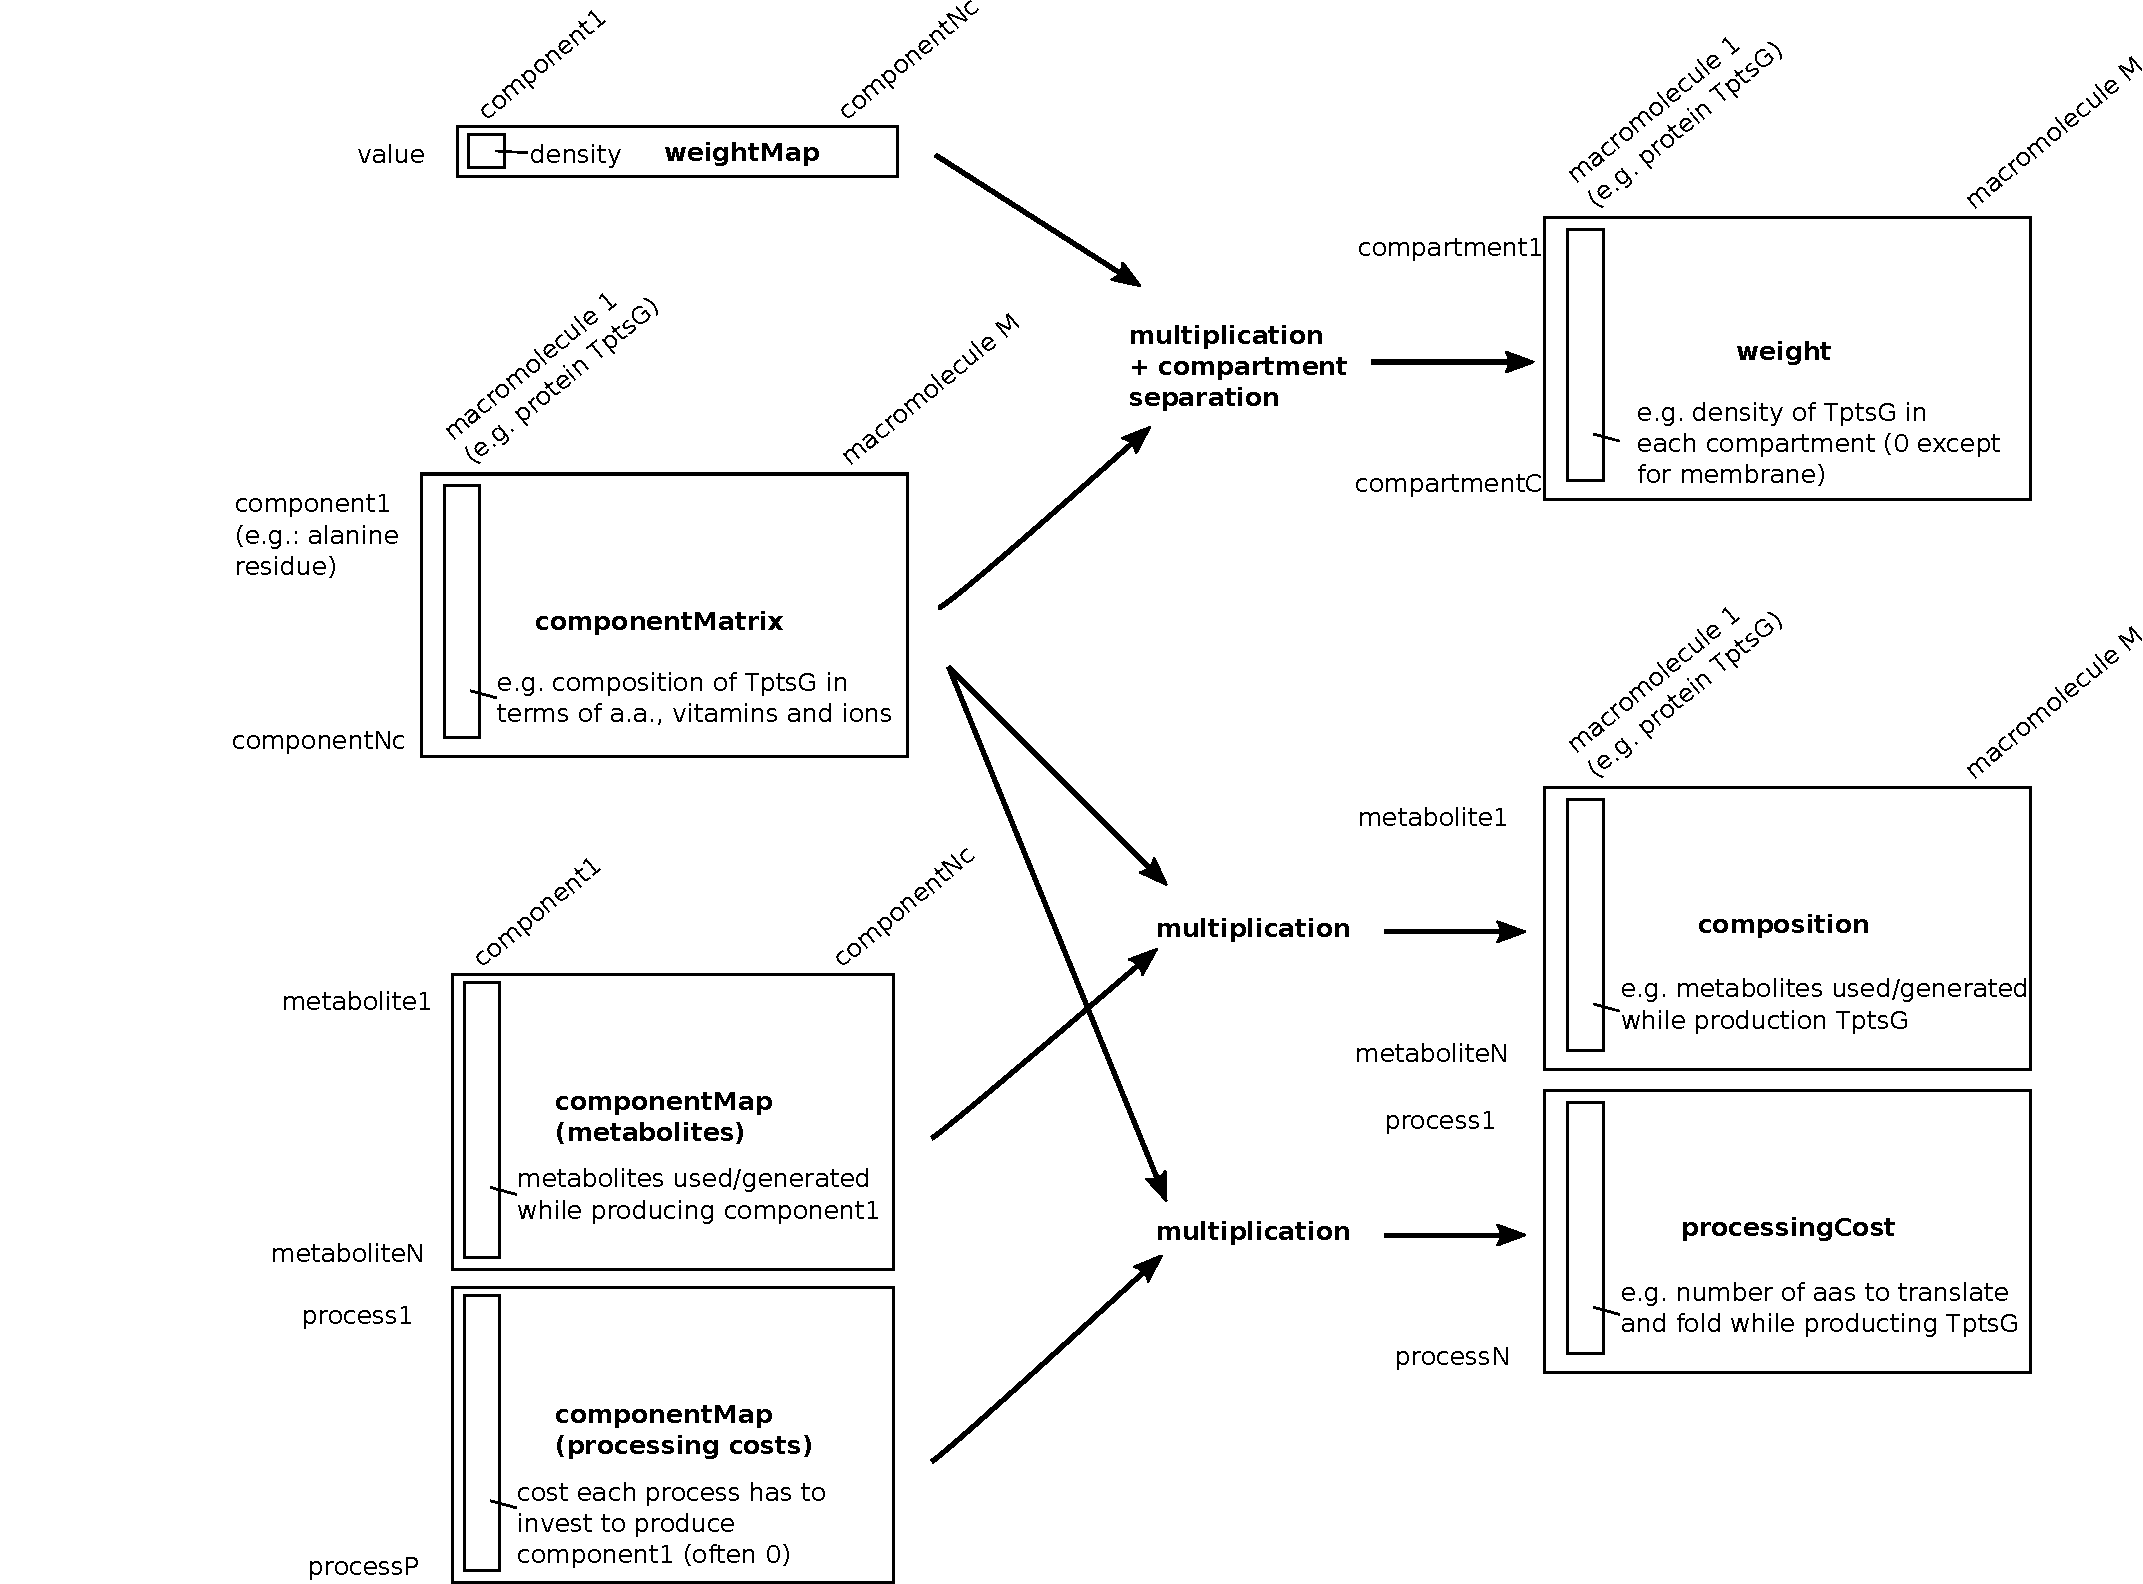
\includegraphics[width=\linewidth]{species_matrices}
  \caption{Matrices extracted from macromolecule information. An example is given with proteins but in the end, they contain all macromolecules and all internal metabolites.}
  \label{fig:species_matrices}
\end{figure}

\paragraph{Machinery matrices} \reffigt{fig:machinery_matrices} shows how the matrices stored in \texttt{rba.processes} are built.
\begin{figure}[ht]
  \centering
  \includegraphics[width=\linewidth]{machinery_matrices}
  \caption{Every machinery can be described by a reaction matrix. Reactants are species (metabolites or macromolecules) needed to build the machinery and products are byproducts of the assembly process. Through matrix multiplication with the species matrices, we can deduce its composition, weight and processing cost.}
  \label{fig:machinery_matrices}
\end{figure}

\paragraph{Target matrices} Targets are either metabolites or macromolecules. Their composition, processing cost and weight can be extracted as columns from the species matrices.
